%!TEX root = ../ArticleCalib_main.tex

%%%%%%%%%%%%% FIGURE 5 : SNR / MODEL HETERO/HOMOG


\begin{figure}[htbp]
\begin{center}
\captionsetup[subfigure]{position=top, labelfont=bf, textfont=normalfont, singlelinecheck=off, justification=raggedright }

\subfloat[]{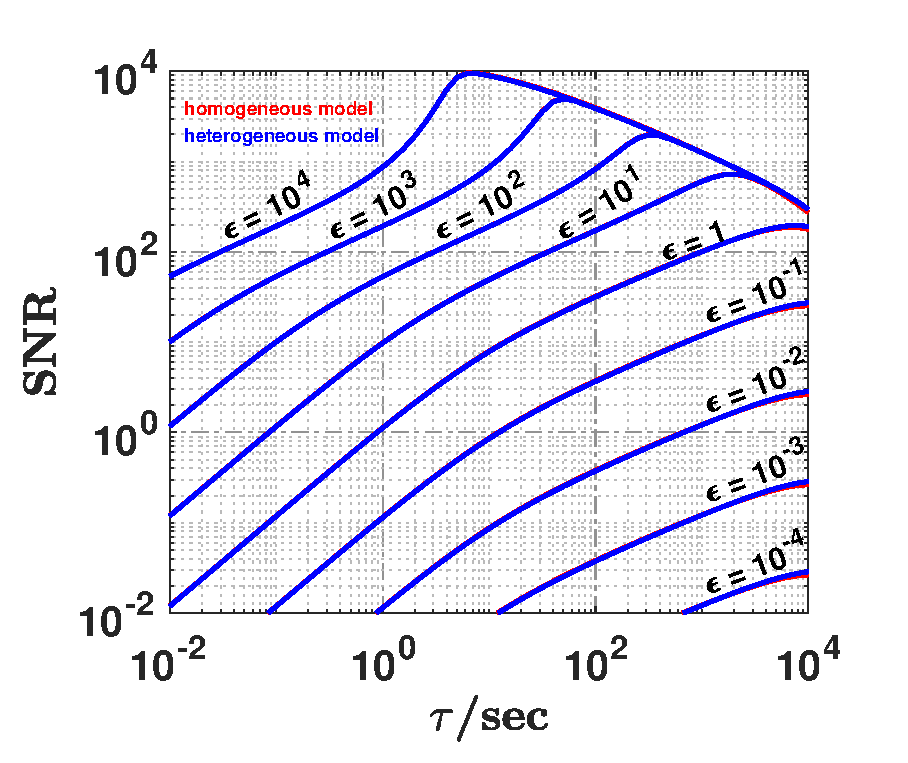
\includegraphics[width=0.4\linewidth]{fig5_compHomoHetero/fig5A_NuvuSimu_E_SNRTau_comparaisonHeteroHomo.eps}\label{fig:SNRTau:HeteroHomo:A}}  \qquad
\subfloat[]{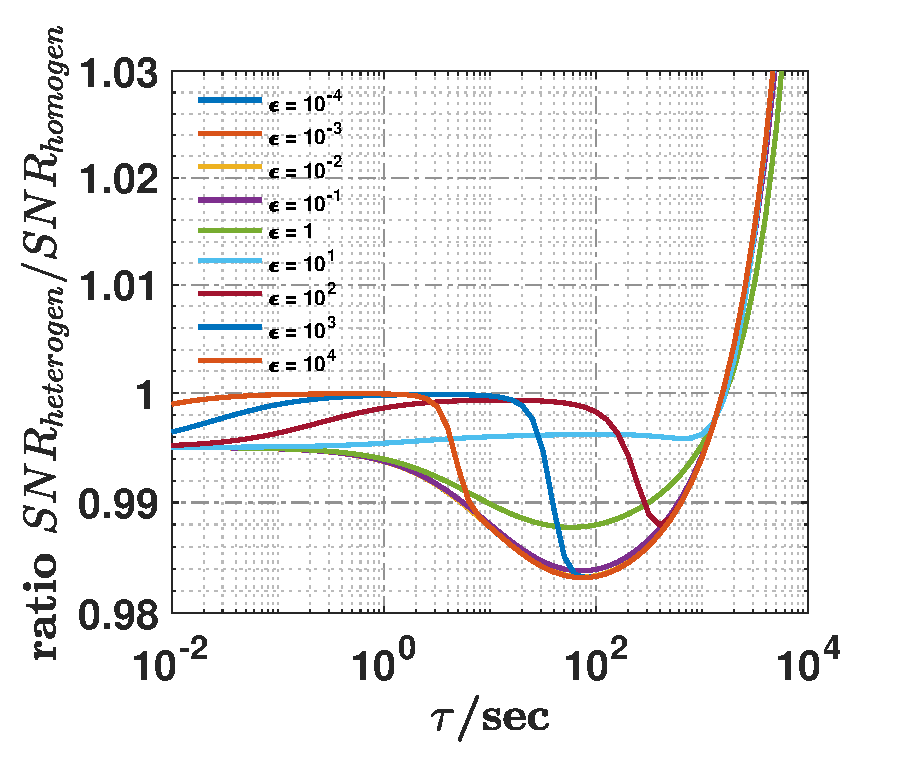
\includegraphics[width=0.4\linewidth]{fig5_compHomoHetero/fig5B_SNR_NuvuSimu_E_SNRTau_ratioHeteroHomo.eps}\label{fig:SNRTau:HeteroHomo:B}}  \qquad


\caption{{\bf SNR models comparaison.} The SNR simulation is represented for different fluxes $\phi$ expressed as a fraction $\epsilon$ of the dark current Id for both the heterogeneous and homogeneous model (\subref{fig:SNRTau:HeteroHomo:A}). The ratio between the SNR for the heterogeneous and homogeneous model is presented in figure \subref{fig:SNRTau:HeteroHomo:B}. }
\label{fig:SNRTau:HeteroHomo}
\end{center}
\end{figure}
%%%%%%%%%%%%%%%%%%%

